%TEX root = ../dissertation.tex

\chapter{Implementation}
\label{chapter:implementation}
In chapter \ref{chapter:solution}, we have presented the solution, that is,
the mobile apps that owners and end users need and the API that developers use
to develop proximity-based mobile apps for this two kinds of users.
Here, it will be explained the implementation of each part of the solution
(tools, programming languages, etc). Since there are two examples that were
created to test the concept, we will dive into their implementation also.
The code is hosted on
github\footnote{http://github.com/}, which is a hosting service for projects
that use git\footnote{http://git-scm.com/}, as their \gls{VCS}.

The technology chosen to support the proximity-based behaviour was
\gls{BLE} Beacons.
We have used three beacons from Estimote\footnote{http://estimote.com}
(figure \ref{fig:estimote}), that come with a development kit.
Besides the hardware, this product offers a \gls{SDK} for Android and
iOS. It also has a cloud service where developers can set and get
some information about each beacon, such as, the \gls{UUID}, name, etc.
% Photo of the three beacons

\begin{figure}[!ht]
  \centering
    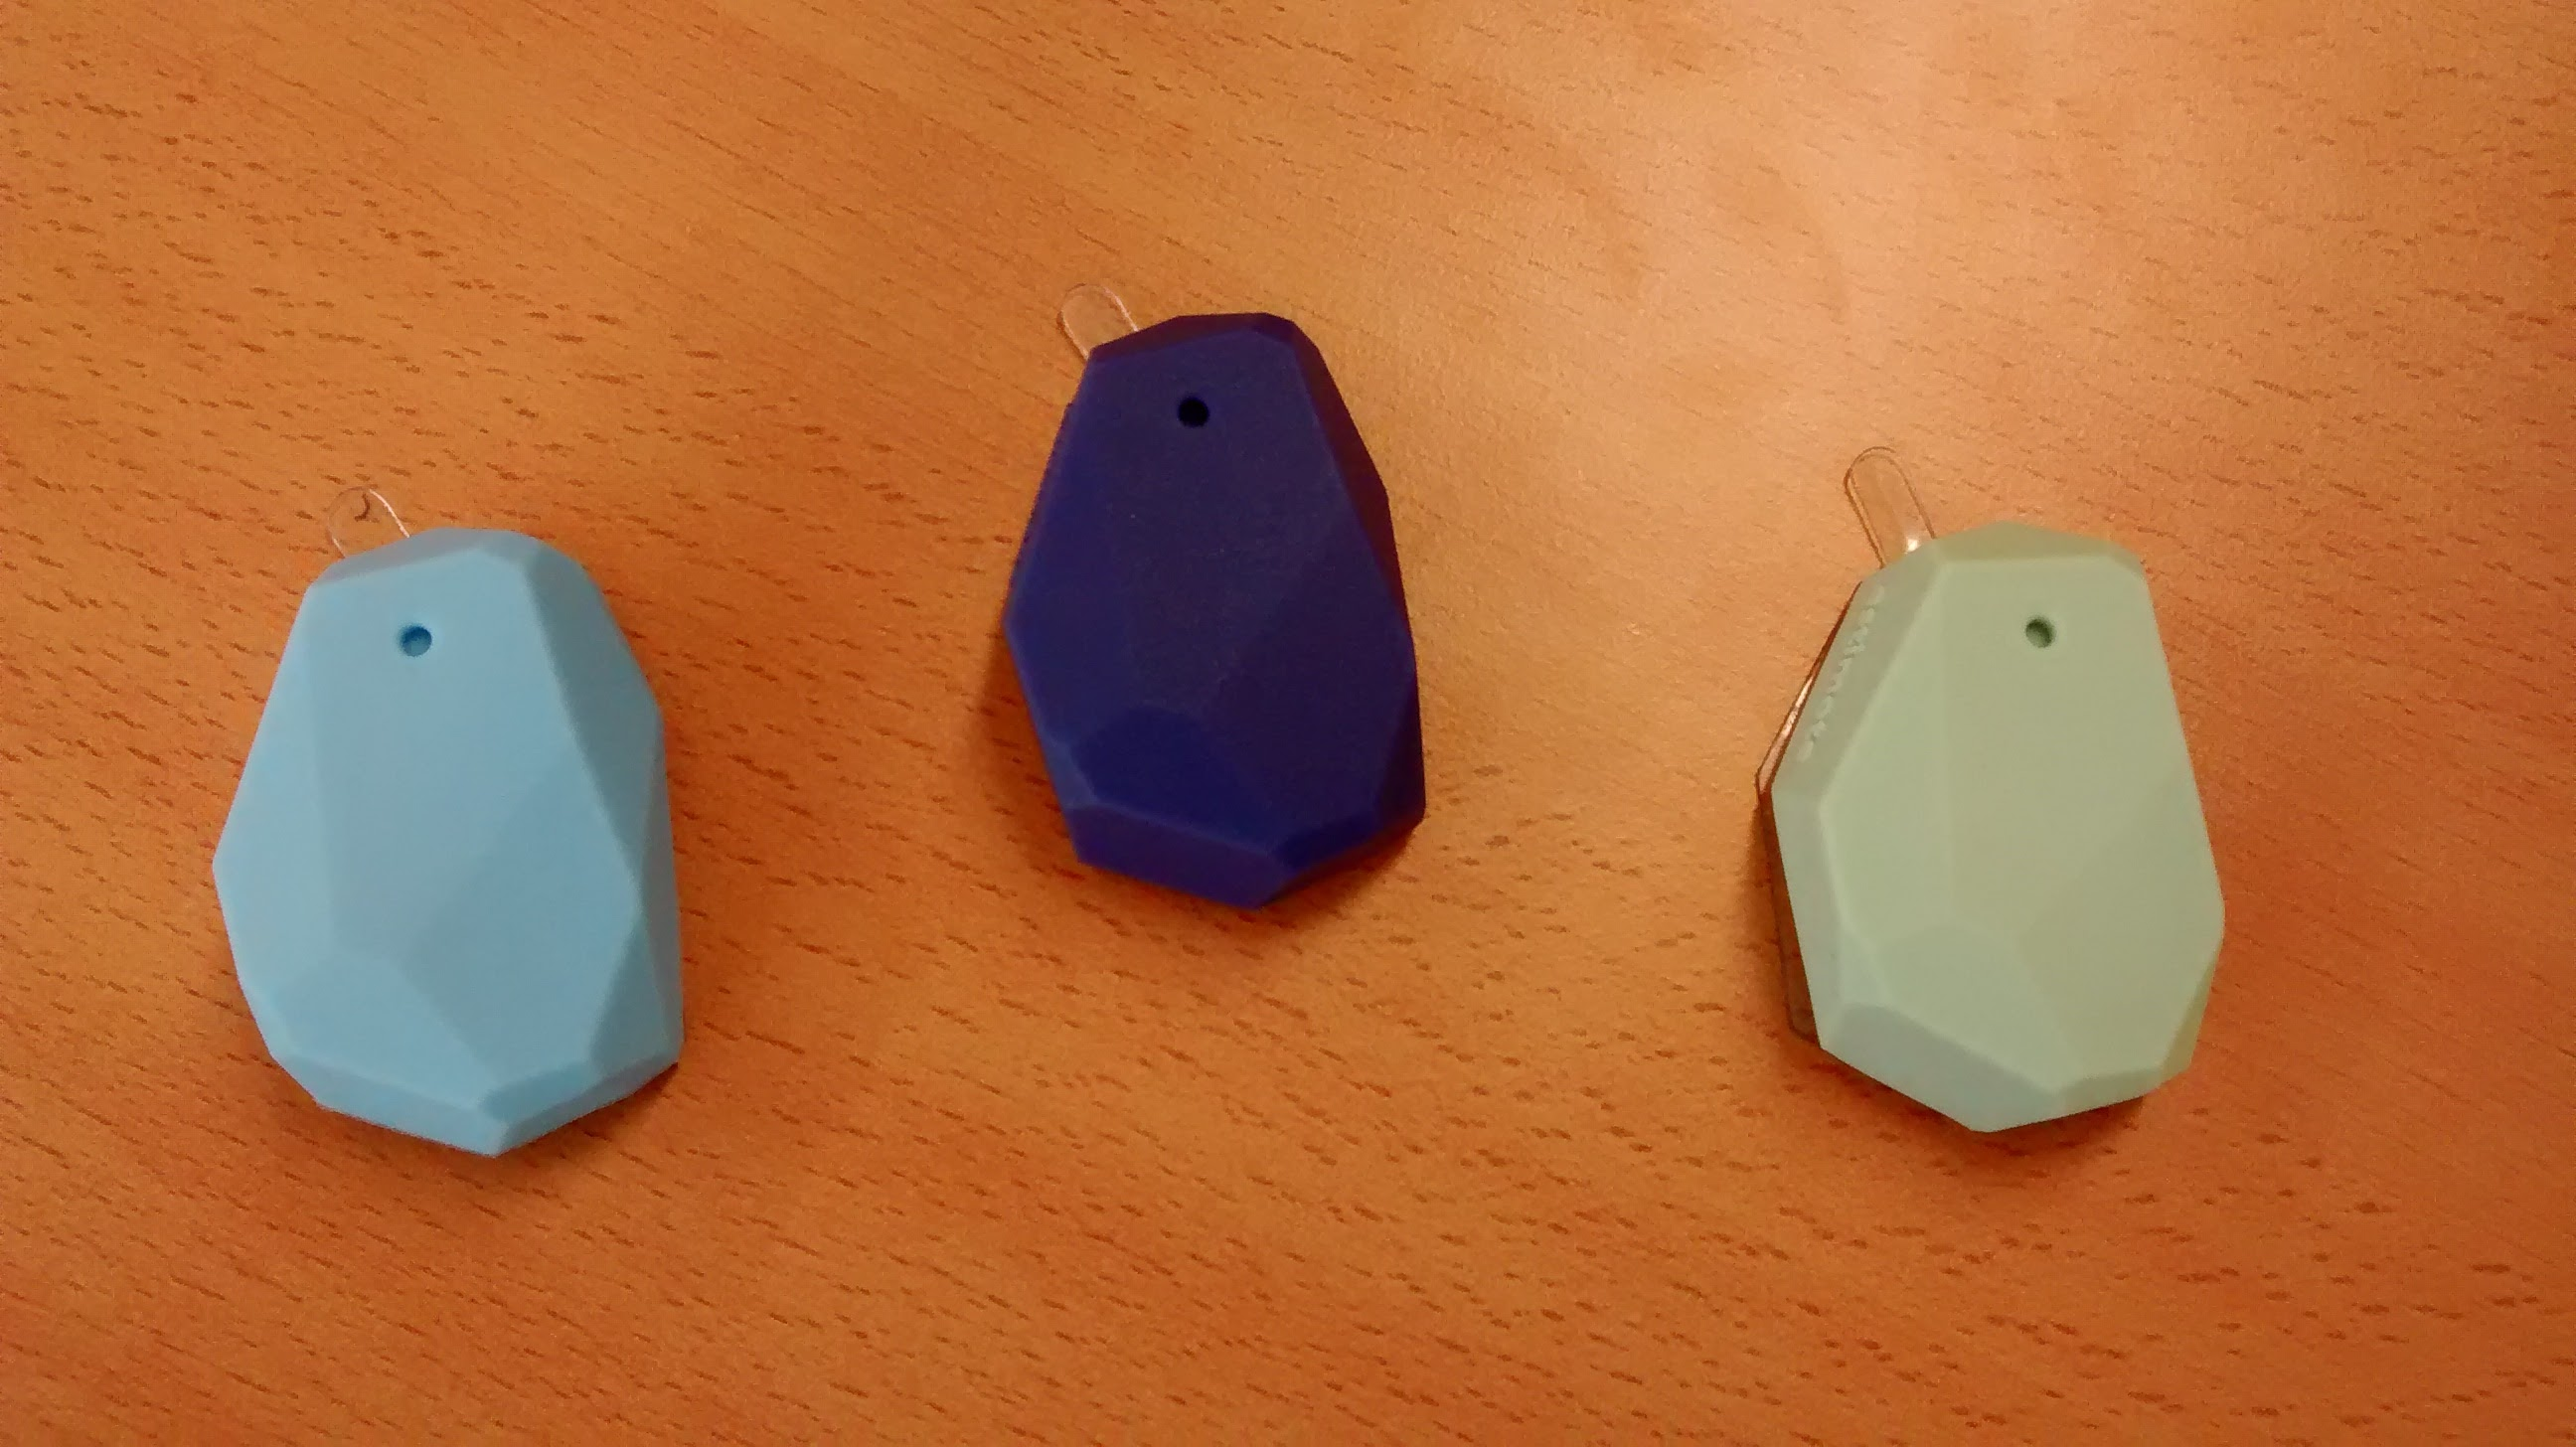
\includegraphics[width=0.5\textwidth, keepaspectratio]{images/estimote}
    \caption{Beacons from Estimote, that were used during the implementation}
    \label{fig:estimote}
\end{figure}

\section{Backend}
\label{sec:backend}
% BaaS, Parse.com
% What it is
% How it works
% Collections created (UML?)
% SDKs used
Since this solution needs to store information about each beacon, we
needed a backend to be able to change this information without having
to change the mobile apps.
However, this backend just had to be able to store data and retrieve that
data when client applications request it.
Instead of implementing this component from the scratch, we used
Parse\footnote{https://parse.com}, which is a \gls{BaaS}.
It gives, to developers, a dashboard, where they can create classes
and define their fields and the type of each field, which can be a string,
a number, a boolean, a pointer to another object, a \gls{JSON} object, etc.
In order to support the needs of this project, the following classes were
created, according to the data model in figure \ref{fig:backend_data_model}:
\begin{description}
  \item[Beacon]: Stores the information according to ibeacon protocol,
  which is \gls{UUID}, major and minor values. It also has a pointer
  to an instance of class User (already provided by Parse.com),
  which represents the user that owns the beacon;
  \item[Smart Place]: Stores information all smart places available,
  such as, name and description. It has a pointer to an instance of
  User, which is the user that created it;
  \item[Smart Place Instance]: When an owner wants to install a given
  Smart Place, he creates an instance of a Smart Place. Owners can
  customize the title and the message that appears in the users'
  mobile devices notifications;
  \item[Tag]: A Tag has a \gls{JSON} object and has pointers to instances
  of Smart Place Instance and Beacon classes. With this pointers, when
  the end users app detects a beacon, it is possible to send a query to
  the backend in order to get the tag that is associated to that beacon.
\end{description}

\begin{figure}[!ht]
  \centering
    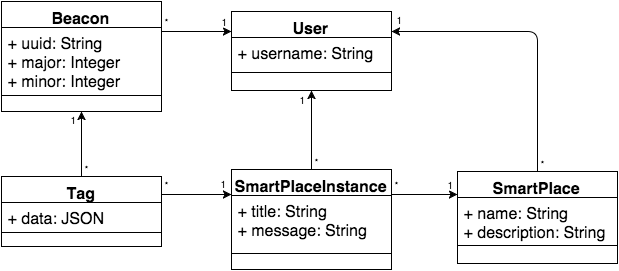
\includegraphics[width=0.5\textwidth]{images/backend_data_model}
    \caption{Data model stored in Parse \gls{BaaS}}
    \label{fig:backend_data_model}
\end{figure}

Parse \gls{BaaS} has \glspl{SDK} available to many platforms and programming
languages, such as, Android, iOS, Javascript, etc.
In order to be able to make requests to the backend from the mobile apps and
from the Javascript API
the Parse Android and Javascript \glspl{SDK} were used.

\section{Mobile applications}
\label{sec:mobile_applications}
% Mobile apps: Tools used, programming languages,
% -> Some kind of UML for each one
There is a mobile app for owners and another one for end users.
Each of these apps is an Android app. They were developed using Android
Studio, which is an \gls{IDE}, based on
IntelliJ\footnote{https://www.jetbrains.com/idea/},
to develop Android
applications and written in JAVA.
The chosen development environment allows developers to create multiple
apps and modules inside the same project.
Taking that into account,
one project was created, with 2 apps and one library, as shown in figure
\ref{fig:smartplaces_package}. Since both apps use the Bluetooth receiver
of the mobile device and make requests to the backend, there is a library,
that both apps depend on, that offers some abstractions around the ibeacon
protocol and the communication with Parse.
Its implementation is detailed in section \ref{sub:library}

\begin{figure}[!ht]
  \centering
    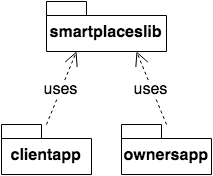
\includegraphics[width=0.5\textwidth, height=0.15\textheight,
      keepaspectratio]{images/smartplaces_package}
    \caption{Android project's structure}
    \label{fig:smartplaces_package}
\end{figure}

\subsection{Library}
\label{sub:library}
% Explain what the lib does
% UML for the lib
% Examples of its usage
As already mentioned, a library, smartplaceslib, was created in order to provide \glspl{API} that mobile apps can
use. Because, both apps use the Bluetooth receiver and interact with the backend, this library avoids having similar code in both apps. There are two important classes that this library offers:
\begin{description}
  \item[IBeaconsManager]: Offers methods to start scanning for beacons and change some settings such as, interval between each scan;
  \item[AbstractParseDataStore]: This class offers an abstraction of the Parse Android \gls{SDK}. It is extended by two classes, ClientParseDataStore, used in the end users mobile app, and OwnerParseDataStore, used in the owners mobile app. There are two different classes for each app because each app has different needs when interacting with the backend. There were common needs encapsulated in methods in the AbstractParseDataStore class.
\end{description}

When IBeaconsManager class is used, it needs a BeaconScanCallback object, which overrides a method that is executed when beacons are scanned, because the scanning is an asynchronous process.
For instance, the following code snippet illustrates how to use IBeaconsManager class, in a given Activity, to scan for nearby beacons.

\begin{lstlisting}
IBeaconsManager manager = new IBeaconsManager(this);
manager.startScan(this, new BeaconScanCallback() {
  @Override
  public void beaconsFound(Collection<BeaconInfo> beacons) {
    // Do something with beacons collection
  }
})
\end{lstlisting}

\subsection{Mobile app for owners}
\label{sub:mobile_app_for_owners}

\subsection{Mobile app for end users}
\label{sub:mobile_app_for_end_users}




\section{Javascript API}
\label{sec:javascript_api}
% JS API
% Tools used (grunt, what is it and tasks used)
% Deployment process (using grunt)
% Make it available as a bower component

\section{Examples}
\label{sec:examples}
% Examples:
% For each one,
% - what it is;
% - tools;
% - programming languages;
% - deployment;
% - overview of its structure

\subsection{Restaurant web application}
\label{sub:restaurant_web_application}

\cite{SLOC}

\subsection{Smart Museum}
\label{sub:smart_museum}
